\let\negmedspace\undefined
\let\negthickspace\undefined
\documentclass[journal]{IEEEtran}
\usepackage[a5paper, margin=10mm, onecolumn]{geometry}
%\usepackage{lmodern} % Ensure lmodern is loaded for pdflatex
\usepackage{tfrupee} % Include tfrupee package

\setlength{\headheight}{1cm} % Set the height of the header box
\setlength{\headsep}{0mm}     % Set the distance between the header box and the top of the text

\usepackage{gvv-book}
\usepackage{gvv}
\usepackage{cite}
\usepackage{amsmath,amssymb,amsfonts,amsthm}
\usepackage{algorithmic}
\usepackage{graphicx}
\usepackage{textcomp}
\usepackage{xcolor}
\usepackage{txfonts}
\usepackage{listings}
\usepackage{enumitem}
\usepackage{mathtools}
\usepackage{gensymb}
\usepackage{comment}
\usepackage[breaklinks=true]{hyperref}
\usepackage{tkz-euclide} 
\usepackage{listings}
% \usepackage{gvv}                                        
\def\inputGnumericTable{}                                 
\usepackage[latin1]{inputenc}                                
\usepackage{color}                                            
\usepackage{array}                                            
\usepackage{longtable}                                       
\usepackage{calc}                                             
\usepackage{multirow}                                         
\usepackage{hhline}                                           
\usepackage{ifthen}                                           
\usepackage{lscape}
\begin{document}

\bibliographystyle{IEEEtran}
\vspace{3cm}
\title{4.4.2.11}
\author{EE24BTECH11032 - John Bobby}
% \maketitle
% \newpage
{\let\newpage\relax\maketitle}

\renewcommand{\thefigure}{\theenumi}
\renewcommand{\thetable}{\theenumi}
\setlength{\intextsep}{10pt} % Space between text and floats


\numberwithin{equation}{enumi}
\numberwithin{figure}{enumi}
\renewcommand{\thetable}{\theenumi}


\textbf{Question:}Find the direction vector and the normal vector for the line $y=3x$\\

\begin{table}[h!]    
  \centering
  \begin{tabular}[12pt]{ |c| c|}
    \hline
        \textbf{Variable}  & \textbf{Description}\\
    \hline
        $a,b$ &  Variables inside the coordinates\\
    \hline 
        $\vec{P}\brak{9a-2,-b}$ & coordinates of point $P$\\
    \hline
	$\vec{A}\brak{3a+1.-3}$ & coordinates of point $A$\\
    \hline
	$\vec{B}\brak{8a,5}$ & coordinates of point $B$\\
    \hline
	$k$ & ratio in which P divides $\vec{AB}$\\
    \hline 
\end{tabular}

  \caption{Input Parameters}
  \label{tab4.4.2.11}
\end{table}

\solution \\
\begin{align}
	y&=3x\\
	\myvec{-3 & 1}\myvec{x\\y}&=0\\
	\vec{n}^\top \vec{x} &=c\\
	\implies \vec{n}&=\myvec{-3\\ 1}\\
	\vec{m}^\top \vec{n} &= 0\\
	\myvec{1 & m}\myvec{-3 \\ 1}&=0\\
	-3+m &=0\\
	\implies m &= 3
\end{align}
the normal vector and the direction vector of the line $y=3x$ can be represented as $\vec{n}$ and $\vec{m}$\\
\begin{align}
	\vec{m} &= \myvec{1\\3},\vec{n} = \myvec{-3\\1}
\end{align}
\begin{figure}[h!]
                \centering
               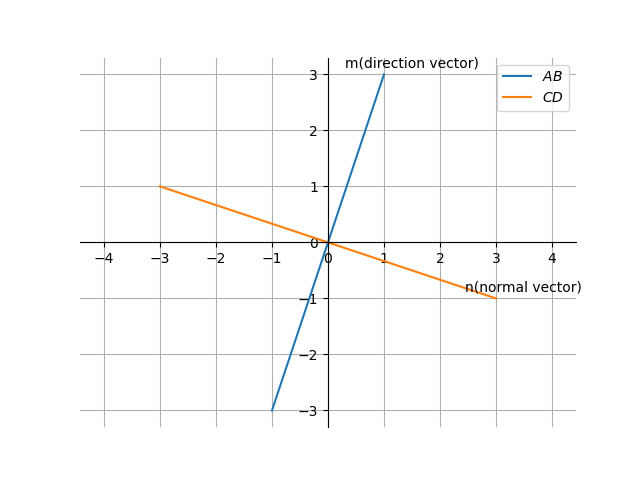
\includegraphics[width=0.7\linewidth]{Figs/Fig1.png}
			\caption{Plot of normal vector and directon vector}
               \label{stemplot}
               \end{figure}


\end{document}
